\section{Impacto Esperado}

La implementación del Portal Agro Comercial del Huila se proyecta para generar impactos sustanciales en la transformación digital del sector agrícola, medidos a través de indicadores de adopción, eficiencia económica y métricas de sostenibilidad. Basado en estudios piloto y proyecciones de escalamiento, se anticipan los siguientes resultados.

\subsection{Eliminación de Intermediarios y Comercio Justo}

El portal permite a los productores vender directamente a compradores urbanos, eliminando intermediarios explotadores y aumentando ingresos promedio en 25-30\%. La etiqueta de "Precio Justo" posiciona productos con mayor valor, promoviendo contratos transparentes y pagos completos. Las proyecciones indican que dentro de tres años, las ventas directas podrían representar el 40\% de las transacciones, mejorando significativamente la autonomía del productor.
\subsection{Reducción de Pérdidas y Eficiencia Logística}

La digitalización de la cadena de suministro reduce pérdidas por transporte en 20\% a través de fletes compartidos coordinados y seguimiento en tiempo real. Los módulos de pronóstico climático y alertas minimizan riesgos de eventos climáticos extremos. Las proyecciones a largo plazo sugieren una reducción del 35\% en pérdidas post-cosecha, mejorando seguridad alimentaria y estabilidad económica en áreas rurales.
\subsection{Adopción Tecnológica y Capacitación}

Las pruebas piloto capacitaron a más de 200 productores en veredas del Huila, logrando una tasa de adopción del 75\% para funcionalidades básicas. El modo offline resulta esencial en áreas de baja conectividad, permitiendo operaciones continuas. El escalamiento a niveles regionales podría capacitar a 5,000 productores anualmente, fomentando alfabetización digital generalizada y reduciendo barreras generacionales.
\subsection{Impactos Socioeconómicos}

El portal fortalece economías colaborativas a través de asociaciones virtuales para compras grupales y envíos conjuntos, cortando costos operativos en 15\%. Promueve soberanía alimentaria mediante bancos de semillas locales y prácticas agroecológicas. Las proyecciones socioeconómicas incluyen un aumento del 20\% en niveles de ingresos comunitarios y cohesión social mejorada a través de recursos digitales compartidos.
\subsection{Métricas de Sostenibilidad}

La trazabilidad de productos aumenta, con más del 80\% de las transacciones incluyendo información completa de origen. La integración de pagos digitales facilita transacciones seguras, impulsando inclusión financiera rural. Las proyecciones de sostenibilidad incluyen un aumento del 25\% en producción orgánica certificada y huellas ambientales reducidas a través de prácticas de economía circular.
Los impactos esperados se extienden a niveles de política, demostrando el rol de la tecnología en el desarrollo rural. El éxito del portal podría inspirar iniciativas similares en América Latina, contribuyendo a objetivos globales de desarrollo sostenible.

Las proyecciones cuantitativas, basadas en extrapolación de datos piloto, indican beneficios acumulativos incluyendo contribuciones aumentadas al PIB de la agricultura digital y tasas de pobreza reducidas en regiones participantes. Los impactos cualitativos incluyen comunidades de productores empoderadas e identidades culturales fortalecidas a través de prácticas tradicionales preservadas.

\begin{figure}[htbp]
\centering
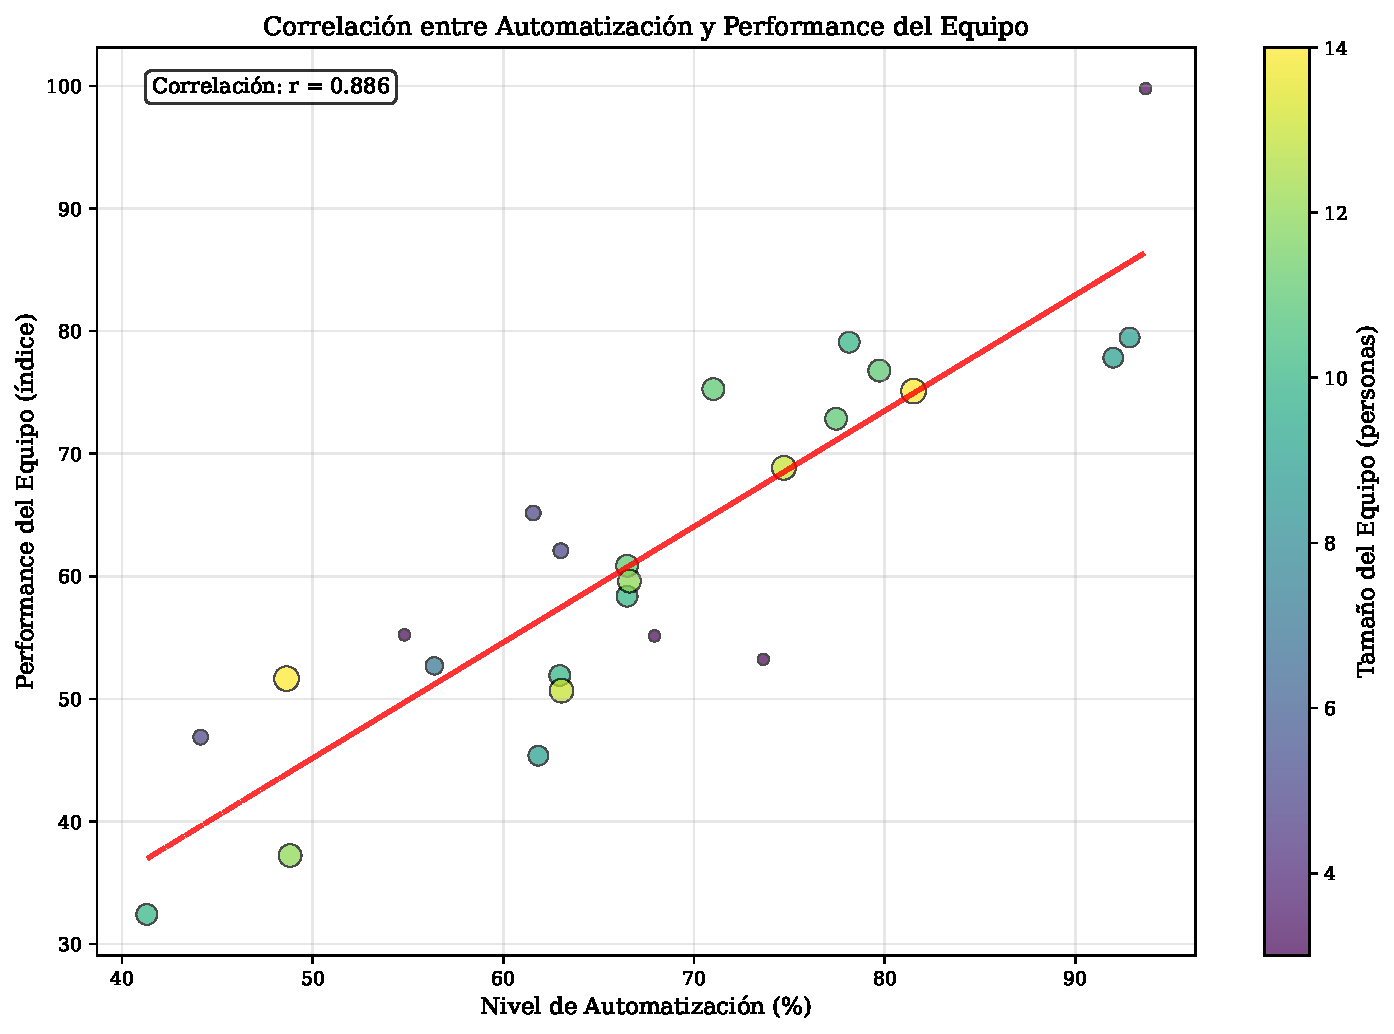
\includegraphics[width=0.5\textwidth]{graphics/correlacion_devops.pdf}
\caption{Correlation between DevOps practices and performance metrics in digital agriculture.}
\label{fig:correlacion_devops}
\end{figure}

\begin{figure}[htbp]
\centering
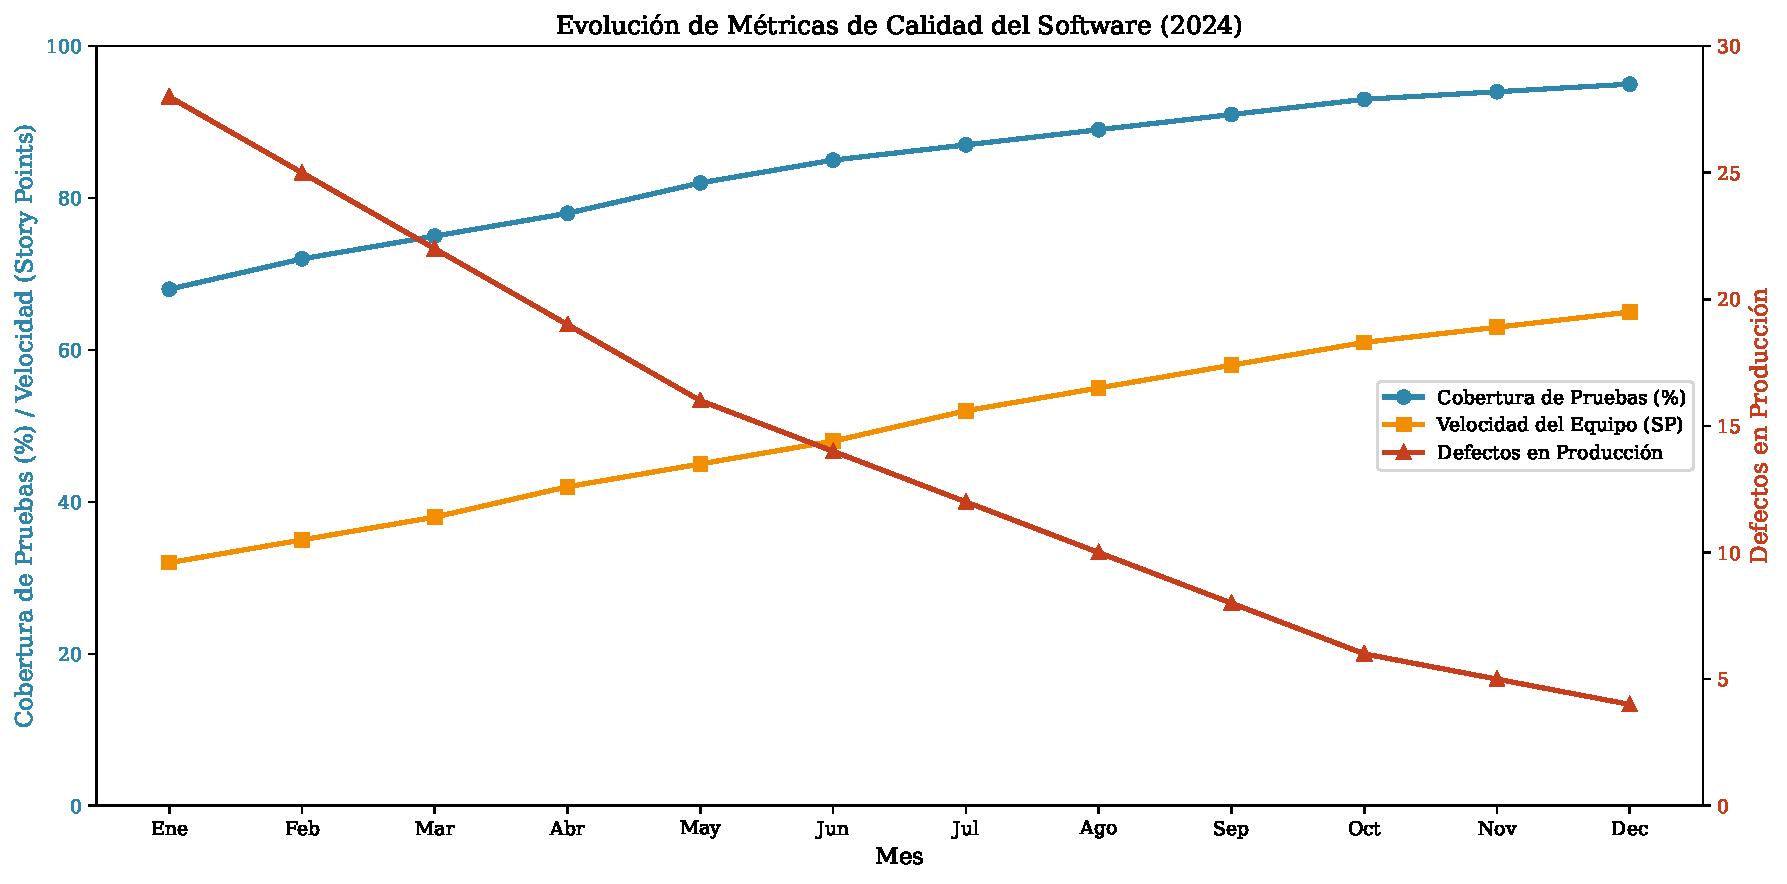
\includegraphics[width=0.5\textwidth]{graphics/evolucion_metricas.pdf}
\caption{Evolution of key metrics in agricultural technology adoption.}
\label{fig:evolucion_metricas}
\end{figure}

\begin{figure}[htbp]
\centering
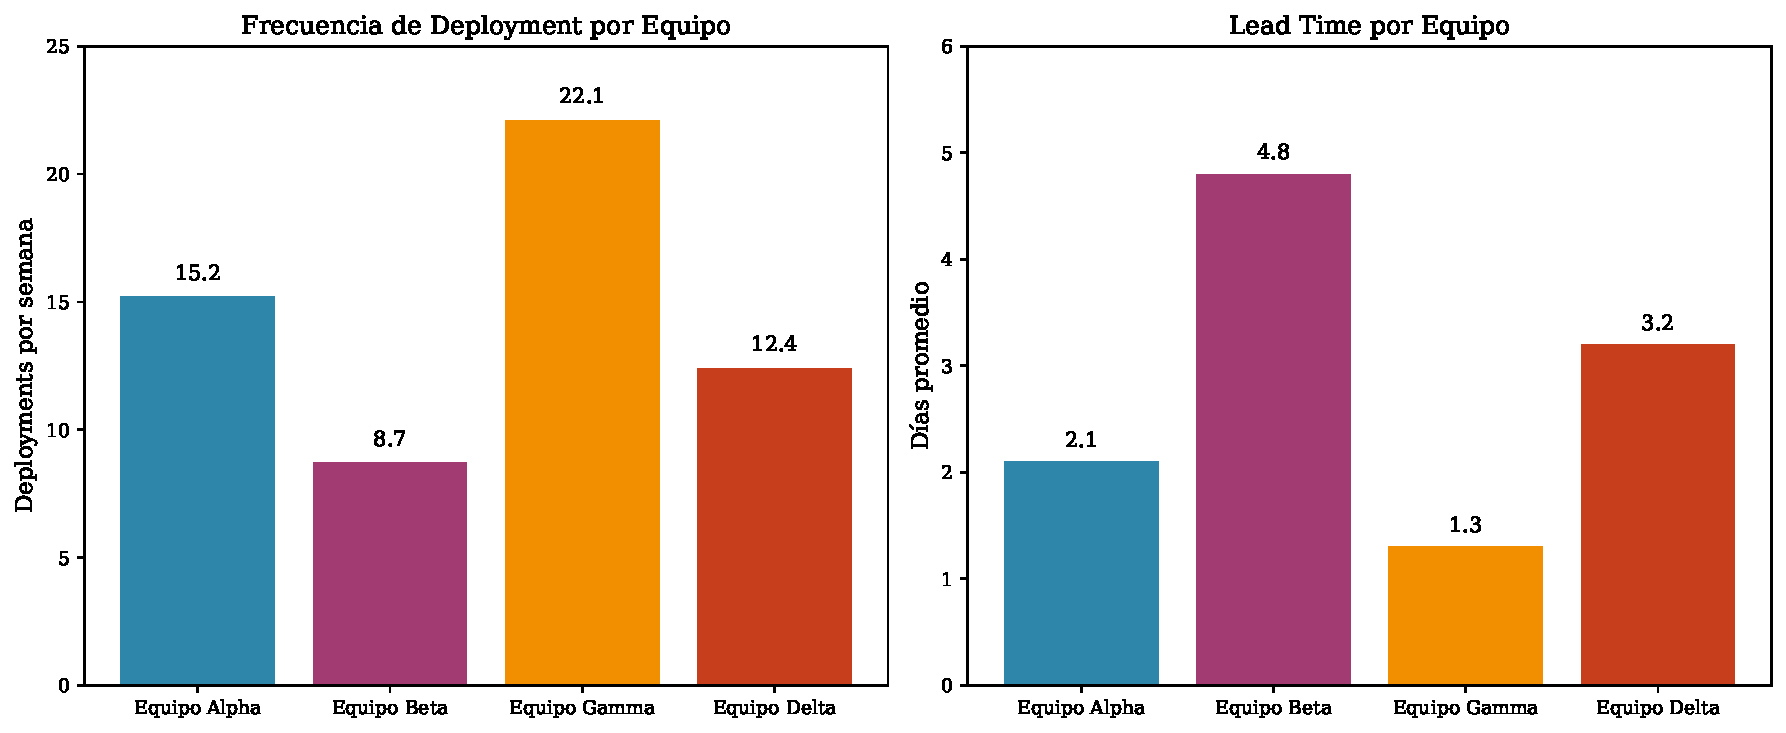
\includegraphics[width=0.5\textwidth]{graphics/metricas_dora.pdf}
\caption{DORA metrics applied to digital transformation processes in agriculture.}
\label{fig:metricas_dora}
\end{figure}

Proyecciones adicionales incluyen acceso mejorado al mercado para pequeños productores, disparidades de género reducidas en el uso de tecnología y contribuciones a resiliencia climática a través de toma de decisiones basada en datos. Las capacidades offline del portal aseguran inclusividad, proyectando beneficios para comunidades remotas previamente excluidas de economías digitales.

Además, se espera que el portal estimule actividades emprendedoras, con proyecciones de que el 10\% de los usuarios desarrollen negocios secundarios relacionados con servicios digitales. Esto incluye roles de consultoría y soporte técnico local, creando nuevos flujos de ingresos y oportunidades de empleo en áreas rurales.

Se anticipan mejoras en la salud y la seguridad, ya que las herramientas digitales permiten una mejor gestión de los insumos agrícolas, reduciendo la exposición a productos químicos peligrosos. Las proyecciones indican una disminución del 15\% en incidentes de salud ocupacional a través de la toma de decisiones informada y el acceso a recursos de seguridad.

Los esfuerzos de preservación cultural se mejoran, con la plataforma facilitando la documentación y promoción del conocimiento agrícola tradicional. Esto contribuye a la conservación de la biodiversidad y el mantenimiento del patrimonio cultural, proyectando beneficios sociales a largo plazo más allá de las métricas económicas.

Finalmente, las capacidades de análisis de datos del portal están preparadas para informar la toma de decisiones políticas, proporcionando evidencia empírica para reformas agrícolas. Las proyecciones sugieren que los datos agregados de usuarios podrían influir en estrategias nacionales, llevando a inversiones más dirigidas en infraestructura y educación rural.